\section{Recasting procedure}
\label{app:recast}

In this appendix we discuss  a general strategy that can be used to reinterpretion existing $t \bar t + \MET$, $b \bar b + \MET$ and $j + \MET$ results obtained in the DMF pseudoscalar model in terms of the \hdma model. Example diagrams that lead to these mono-$X$ signatures in the \hdma model are displayed Figure~\ref{fig:nonresonant}. Notice that only graphs involving the exchange of an $a$ are depicted in this figure but similar diagrams  with an  $A$ are not explicitly shown. 

\begin{figure}[t!]
\centering
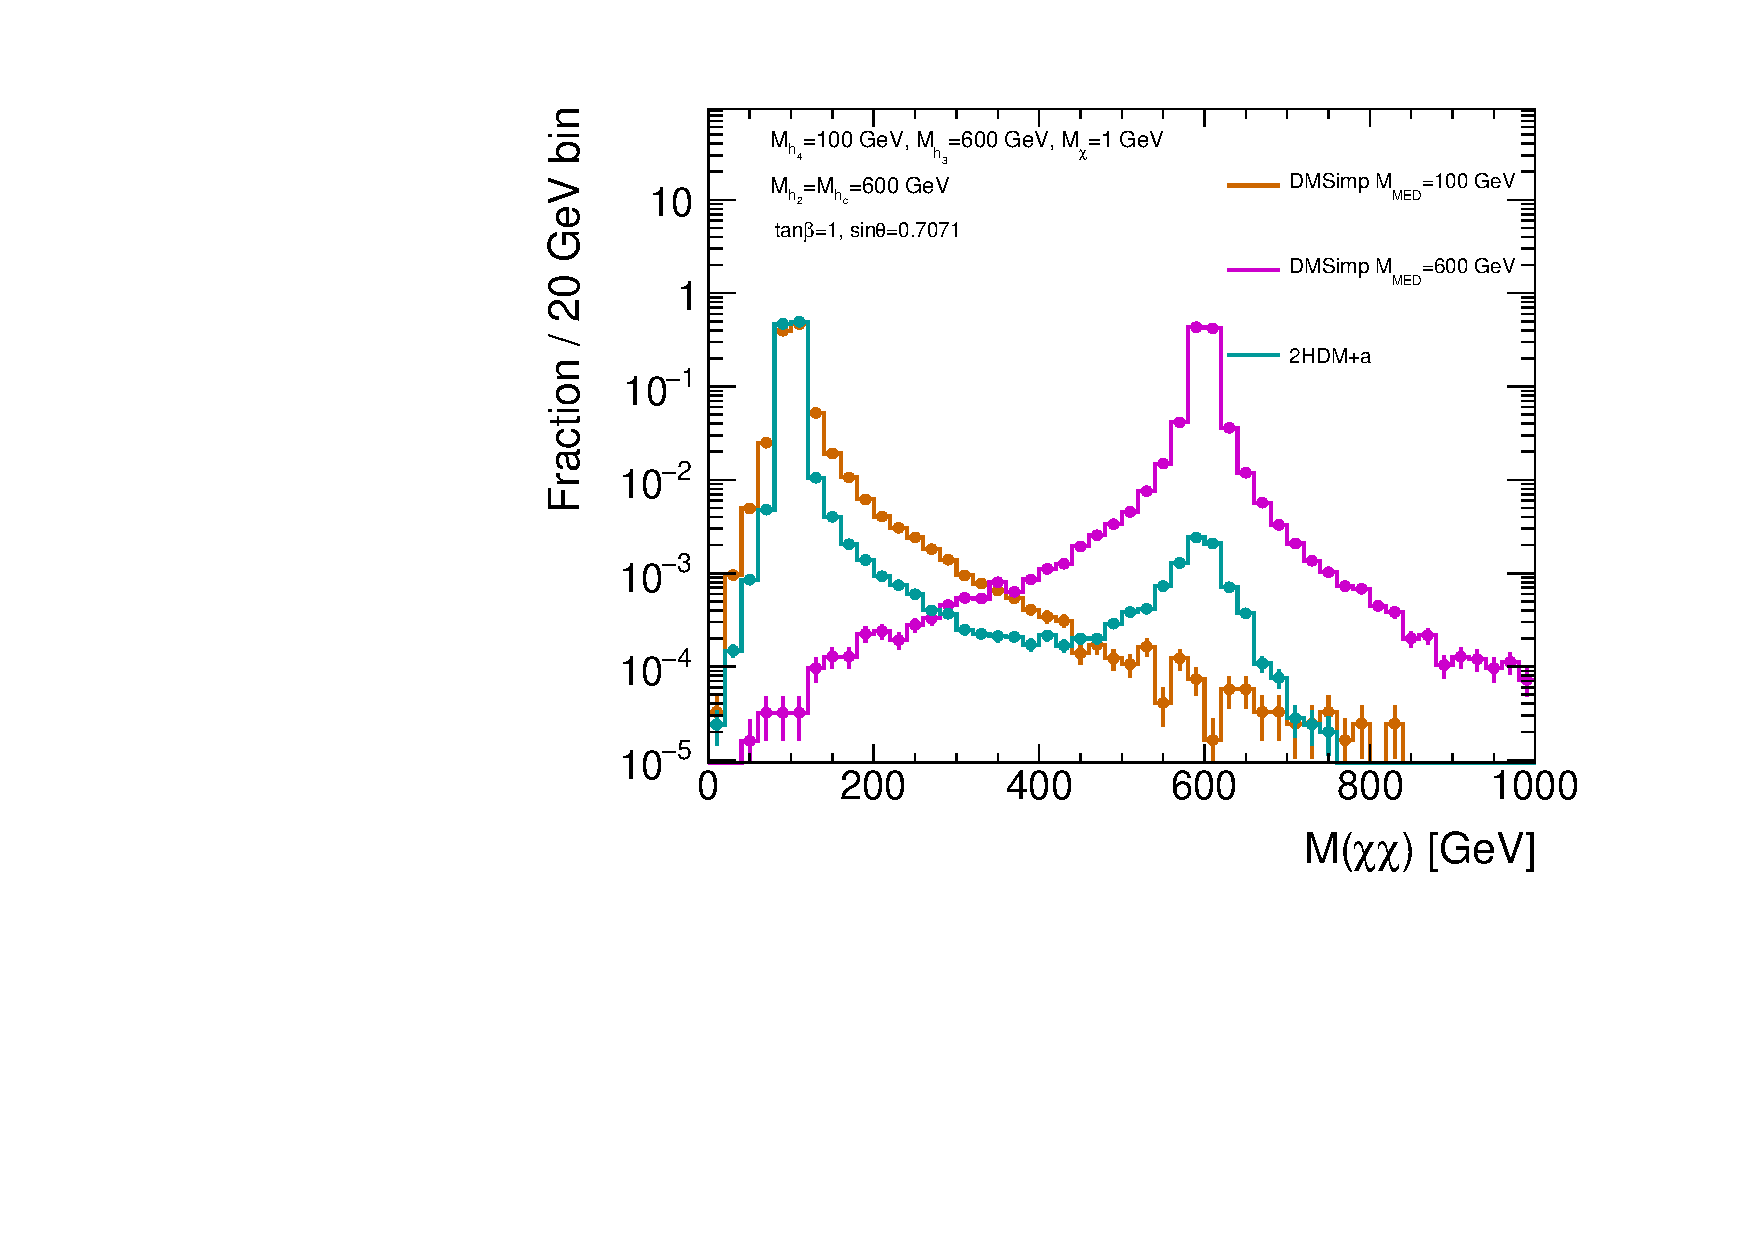
\includegraphics[width=0.5\textwidth]{texinputs/04_grid/figures/DMHF/benchmarking/MDM_1_Ma_100_MA_600_sinp_0.7071_tanb_1.0_VS_DMSimp_100_600_Decayed/mchichi.pdf}
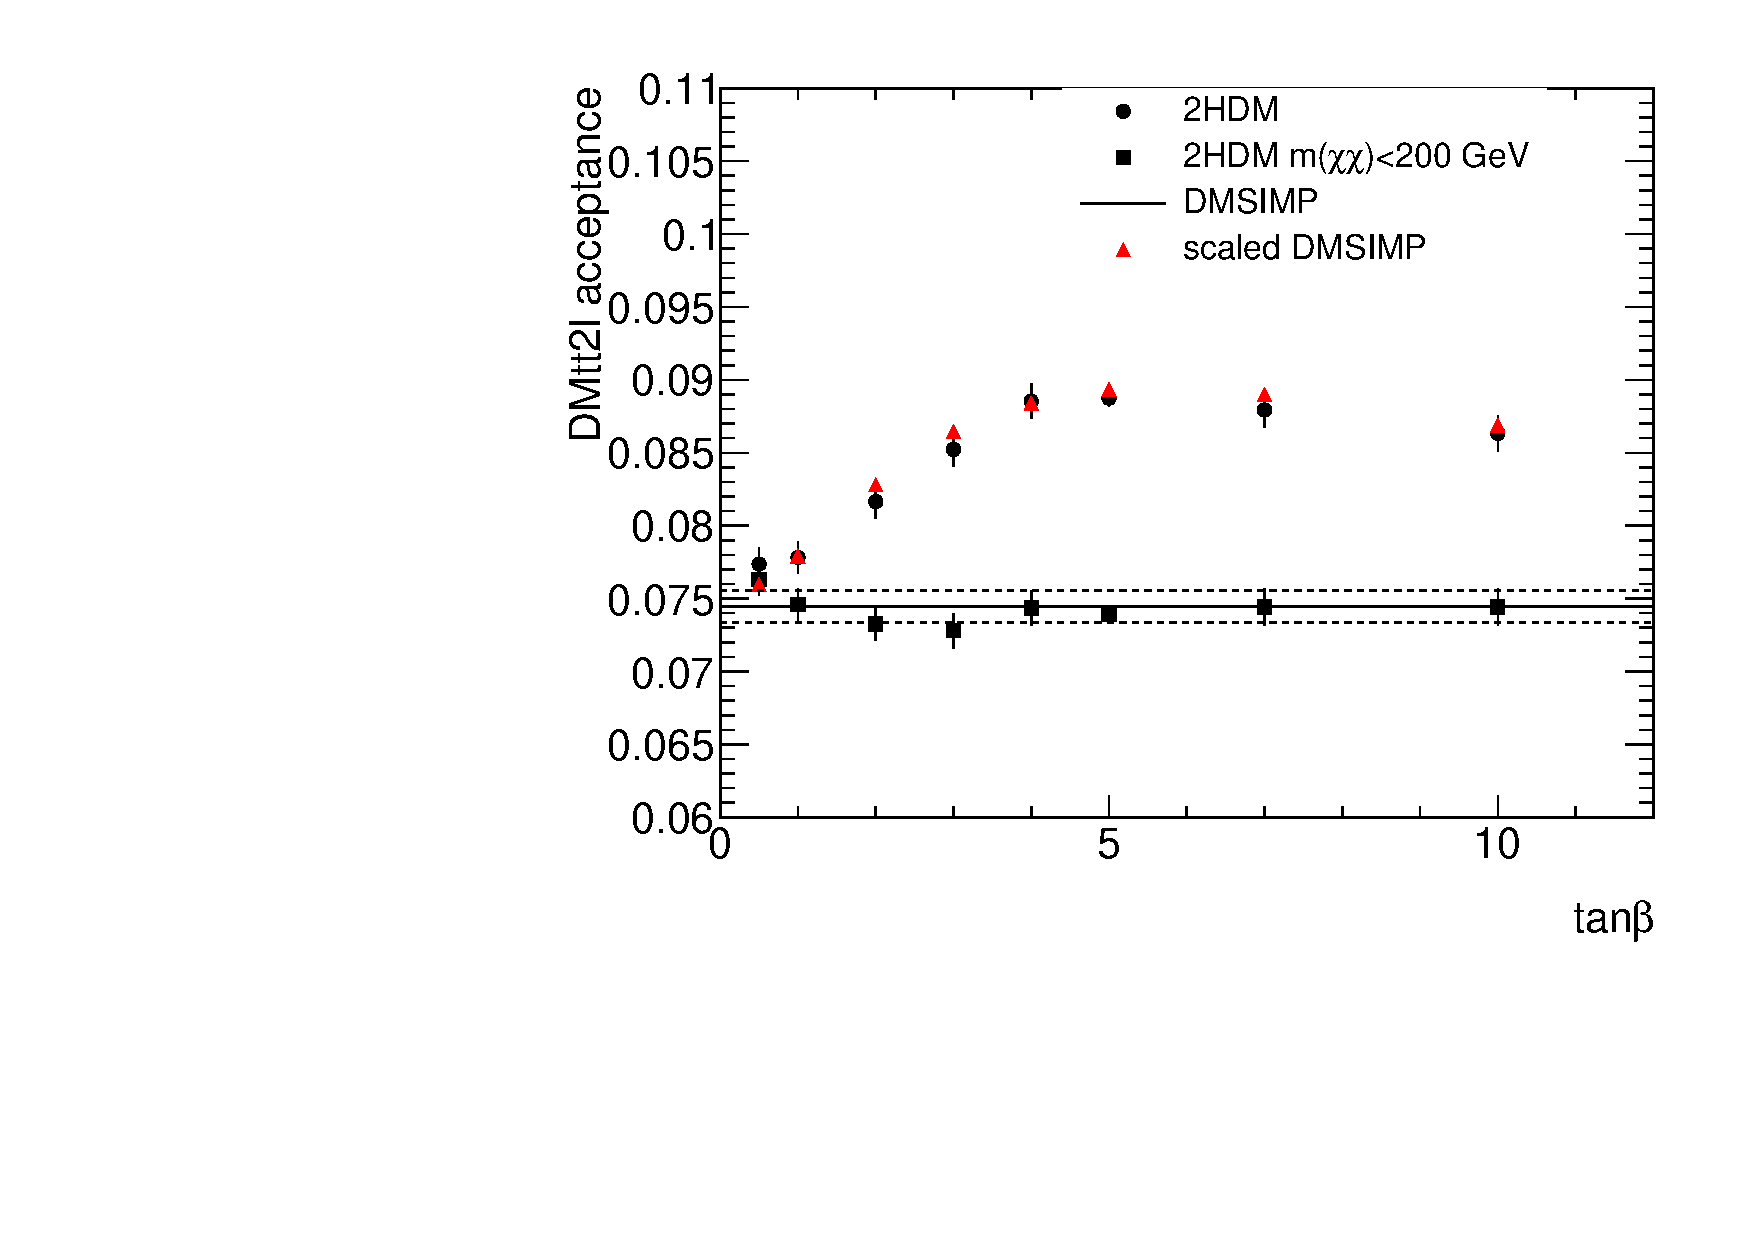
\includegraphics[width=0.45\textwidth]{texinputs/04_grid/figures/DMHF/plotacc_tb.pdf}
\vspace{2mm}
\caption{ \label{fig:mchichi_DMsimpV2HDMa}
Left: Invariant mass of the $\chi\bar{\chi}$ system in $t \bar t + \MET$ production for the DMF pseudoscalar model with $\ma =100 \, {\rm  GeV}$~(brown) and $\ma =600 \, {\rm  GeV}$~(magenta) compared to the \hdma model with $\ma = 100 \, {\rm  GeV}$, $\mH = \mA = \mHc = 600 \, {\rm  GeV}$, $\sin\theta=0.7071$ and $\tan\beta=1$~(cyan). Right: Acceptances of the   two-lepton $t \bar t + \MET$ analysis~\cite{Aaboud:2017rzf}  as a function of $\tan\beta$.  Shown are the predictions in the \hdma model without (round black markers) and with the cut $m_{\chi \bar \chi} <200 \, {\rm GeV}$ (square black markers), assuming $\ma = 150 \, {\rm GeV}$, $\mH= \mA = \mHc = 600 \, {\rm GeV}$ and $\sin\theta=0.35$. The DMF pseudoscalar model result (full black line) with its statistical uncertainty (dashed black lines) as well as the acceptance  ${\cal A}_{\hdma} \left (\ma, \mA \right )$ (red triangles) as defined in~\eqref{eq:recast} is also depicted. {\color{red} [Uli: Fix notation etc.!]}
}
\end{figure}

The relevance of the contributions from both the $a$ and $A$ in the \hdma model can be nicely demonstrated by considering the invariant mass $m_{\chi \bar \chi}$ of the $\chi \bar \chi$ system. Examples of~$m_{\chi \bar \chi}$ distributions in $t \bar t + \MET$ production are shown in the left panel of Figure~\ref{fig:mchichi_DMsimpV2HDMa}. The brown (magenta) histogram corresponds to the prediction in the DMF pseudoscalar model assuming a mediator mass of $\ma =100 \, {\rm  GeV}$ ($\ma =600 \, {\rm  GeV}$), while the cyan histogram illustrates the result in the \hdma model for the choices $\ma = 100 \, {\rm  GeV}$, $\mH = \mA = \mHc = 600 \, {\rm  GeV}$, $\sin\theta=0.7071$ and $\tan\beta=1$. One observes that the predictions obtained in the  DMF pseudoscalar model both show a single  Breit-Wigner  peak  at $m_{\chi \bar \chi} = \ma$, which corresponds to the on-shell production of the mediator $a$ that subsequently decays to a pair of DM particles. The \hdma result instead features two mass peaks, one at $m_{\chi \bar \chi} = \ma$ and another one at $m_{\chi \bar \chi} = \mA$, because both pseudoscalars can be produced on-shell and then decay invisibly via either $a \to \chi \bar \chi$ or $A \to \chi \bar \chi$.  

The above discussion suggests that once the contributions from $a$ and $A$ production are separated, $t \bar t + \MET$, $b \bar b + \MET$ and $j + \MET$  results obtained in the DMF pseudoscalar model can be mapped into the $\hdma$ parameter space. In practice, the remapping is achieved by calculating the selection acceptances~${\cal A}_{\rm DMF} \left ( \ma \right )$ and~${\cal A}_{\rm DMF} \left ( \mA \right )$ in the DMF pseudoscalar model and the respective cross sections~$\sigma_{a, {\rm DMF}}$ and~$\sigma_{A, {\rm DMF}}$. The acceptance~${\cal A}_{\hdma} \left (\ma, \mA \right )$ in the \hdma model  is then obtained by computing the following weighted average
\begin{equation} \label{eq:recast}
{\cal A}_{\hdma} \left (\ma, \mA \right )=\frac{ {\cal A}_{\rm DMF} \left ( \ma \right )\, \sigma_{a, {\rm DMF}} + {\cal A}_{\rm DMF} \left ( \mA \right ) \, \sigma_{A, {\rm DMF}} }{\sigma_{a, {\rm DMF}}+\sigma_{A, {\rm DMF}}} \,.
\end{equation}

\begin{figure}[t!]
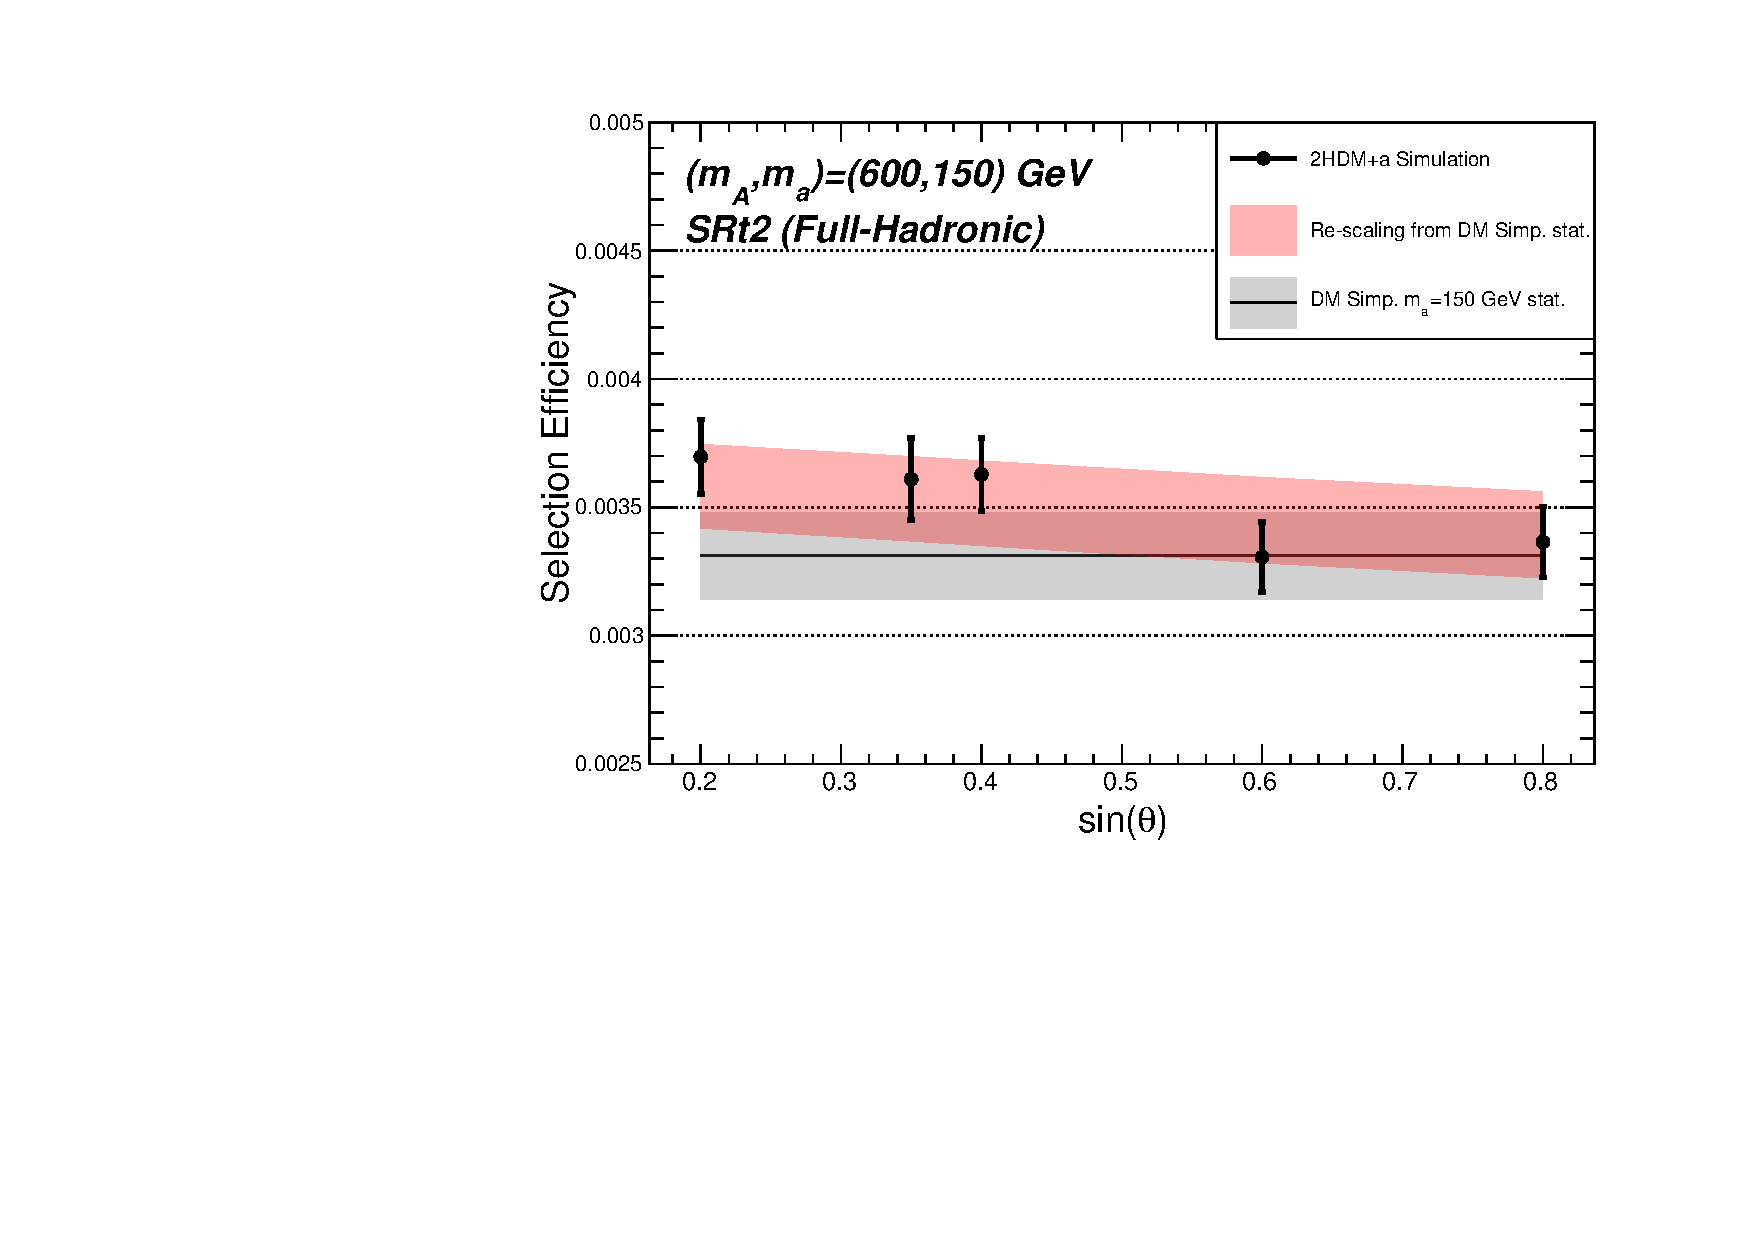
\includegraphics[width=.5\textwidth]{texinputs/04_grid/figures/DMHF/SRt2_600_150_sin}
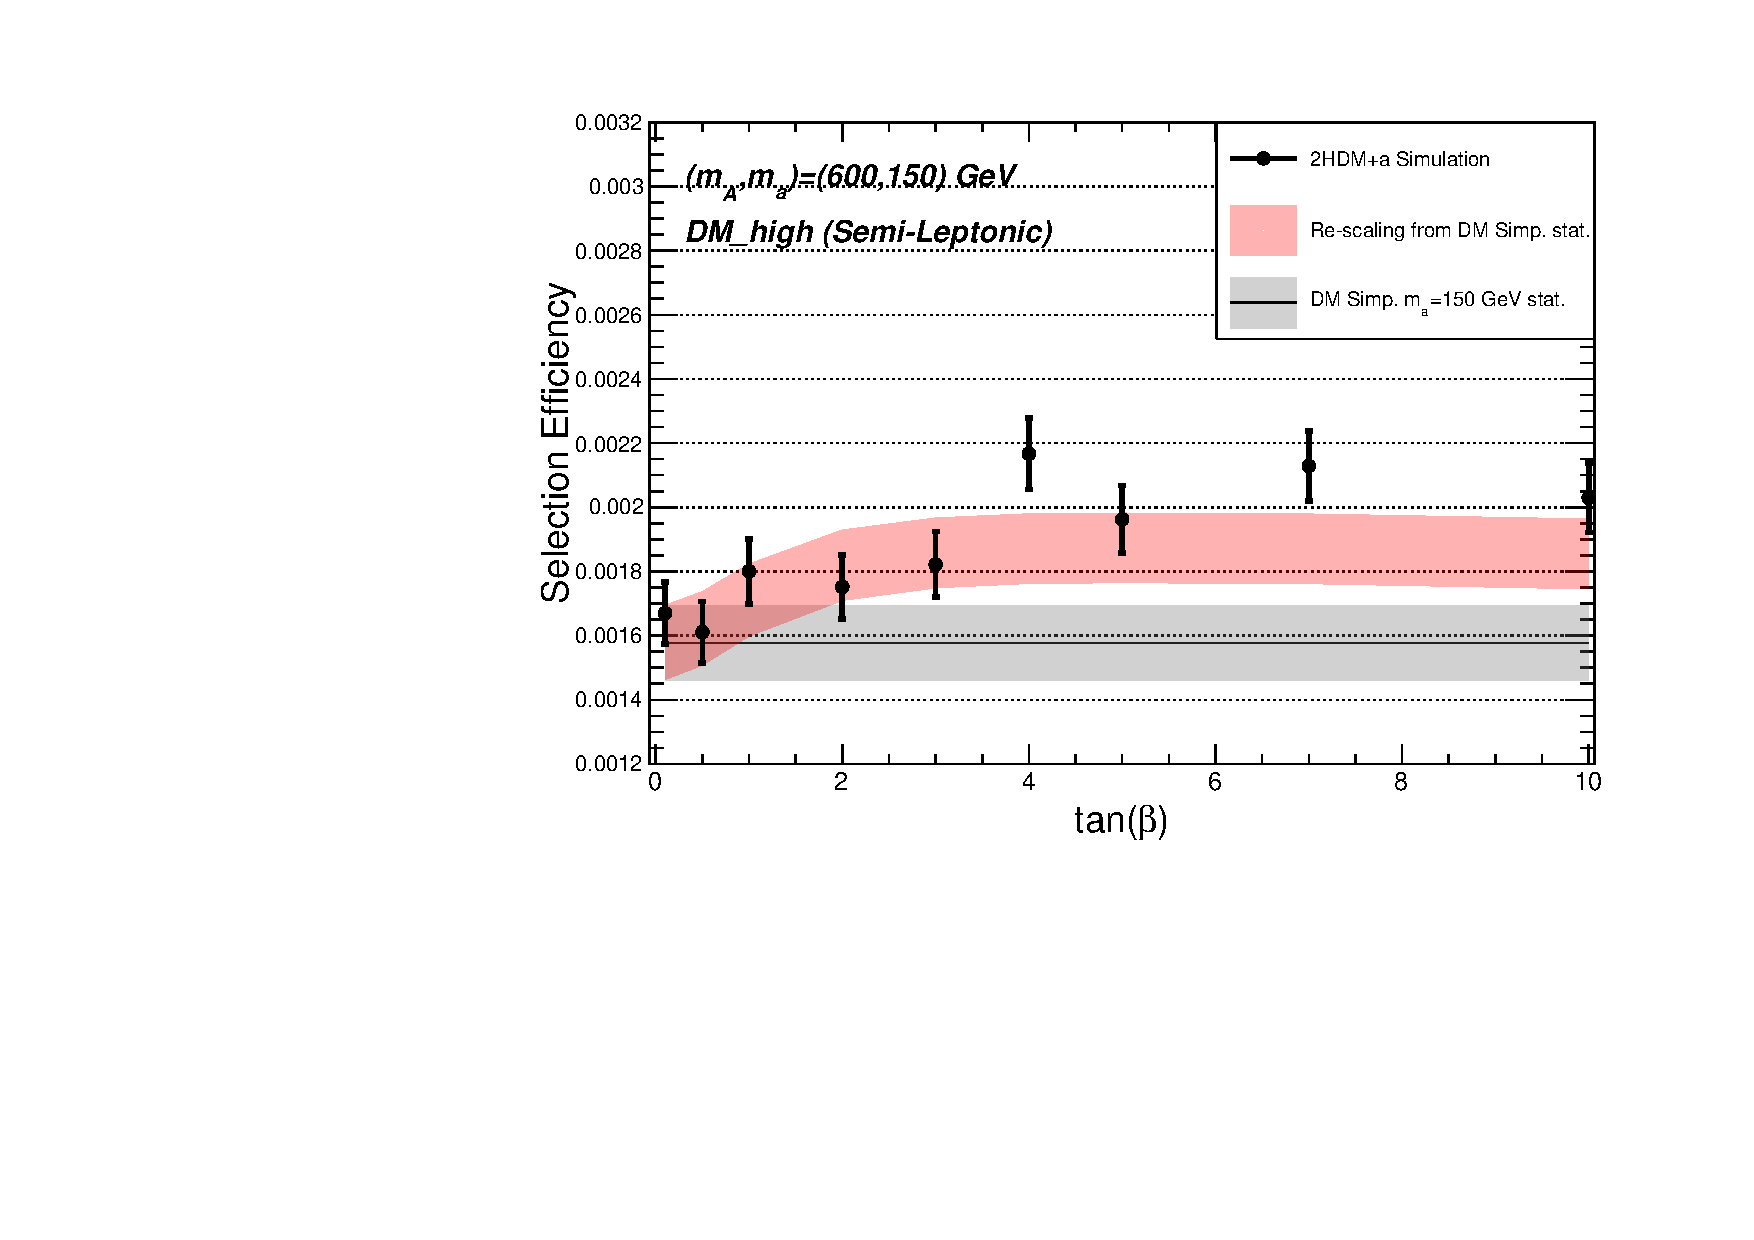
\includegraphics[width=.5\textwidth]{texinputs/04_grid/figures/DMHF/DM_high_600_150_tan}
\vspace{2mm}
\caption{Validation of~\eqref{eq:recast} in the case of the hadronic (left panel) and the one-lepton (right panel)  final state arising from the $t \bar t+\MET$ signature. The direct \hdma calculations are indicated by the black dots and error bars, while the grey and red bands indicate the result in the DMF pseudoscalar model and the prediction obtained using the rescaling formula.  In the left (right) panel, the  chosen parameters are $\ma = 150 \, {\rm GeV}$, $\mH= \mA = \mHc = 600 \, {\rm GeV}$ and $\tan \beta = 1$ ($\sin\theta=0.35$).  {\color{red} [Uli: Correct? Fix notation etc.!]}}
\label{DMHF:pof}
\end{figure}

In the right panel of Figure~\ref{fig:mchichi_DMsimpV2HDMa} we show the results that are obtained by applying the latter equation to a parton-level implementation of the two-lepton $t \bar t + \MET$ analysis described in~\cite{Aaboud:2017rzf}. The round (square) black markers indicate the results of a direct calculation in the \hdma model without a $m_{\chi \chi}$ cut (imposing the cut $m_{\chi \bar \chi} < 200 \, {\rm GeV}$), using $\ma = 150 \, {\rm GeV}$, $\mH= \mA = \mHc =600 \, {\rm GeV}$ and $\sin\theta=0.35$. The DMF pseudoscalar model result with its statistical uncertainty is represented by the solid and dashed black lines. The acceptance calculated from \eqref{eq:recast} is finally indicated by the red triangles. Two features are evident from the figure. First, the \hdma acceptance with cut agrees with uncertainties with the acceptance of the DMF pseudoscalar model. This is expected because the cut $m_{\chi \bar \chi} < 200 \, {\rm GeV}$ strongly suppresses the $A$ contribution in the \hdma model. Second, the acceptance estimated using  \eqref{eq:recast} agrees within uncertainties with the acceptance evaluated directly in the \hdma sample. 

Further validations of~\eqref{eq:recast} are presented in Figure~\ref{DMHF:pof}. In this figure we apply the rescaling formula to the case of the   hadronic~\cite{Aaboud:2017rzf} (left panel) and the one-lepton~\cite{Aaboud:2017aeu}~(right panel)  final state arising in the context of $t \bar t+\MET$ production. The direct \hdma calculations are indicated by the black dots and error bars, while the grey and red bands illustrate the result in the DMF pseudoscalar model and the prediction obtained using~\eqref{eq:recast}. In the left (right) panel, we have employed $\ma = 150 \, {\rm GeV}$, $\mH= \mA = \mHc = 600 \, {\rm GeV}$ and $\tan \beta = 1$ ($\sin\theta=0.35$). One observes that the rescaled results describe the $\sin \theta$ and $\tan \beta$ dependence of the \hdma result well. {\color{red} [Uli: In fact, not an amazing agreement!]} We finally add that the formula~\eqref{eq:recast} has also been successfully tested in the case that $|\mA - \ma| \simeq 50 \, {\rm GeV}$, in which case the interference between the $a$ and $A$ contributions is phenomenologically relevant.  





 
